\documentclass[
	msc, %% Para dissertações de mestrado, OU
%	mscproposta, %% Para propostas de dissertação de mestrado, OU
	% phd, %% Para teses de doutorado, OU
%	phdproposta, %% Para propostas de tese de doutorado
	portugues %% Para documentos em português, OU
	% english %% Para documentos em inglês
]{../ppgccufmg}

% \usepackage{etoolbox} % Adicione este pacote para supressão do erro

% Exemplo de substituição de \addtodef
% \addtodef{\command}{<before>}{<after>}
\pretocmd{\command}{<before>}{}{}
\apptocmd{\command}{<after>}{}{}

\usepackage[brazil]{babel}
 %% se o documento for em português, OU
\usepackage{hyphenat}

% \usepackage[english]{babel} %% se o documento for em inglês
%\usepackage[latin1]{inputenc}
\usepackage{natbib}
\usepackage{xcolor}
\usepackage{lipsum}
\usepackage{url}
\usepackage{amsmath, amssymb}
\usepackage{graphicx}
\usepackage{float}

\usepackage[
	colorlinks=true, 
	linkcolor=blue, %% Cor dos links do sumário
	citecolor=red, %% Cor dos links das citações      
	urlcolor=magenta, %% Cor das urls
]{hyperref}

%% Exemplo 1 de lista customizada: Glossário ==================

\newcommand{\glossario}{
	\chapter*{List of Abbreviations and Acronyms}
	
	\begin{tabular}{ll}
		BFS & \textit{Breadth-First Search}\\
		BOW & \textit{Bag of Words} \\
		TXT & \textit{Text File Format}\\
		UFMG & Universidade Federal de Minas Gerais
	\end{tabular}
}

%% **** Caso não haja nenhuma lista adicional, os comandos acima podem ser apagados. ****
%% ===============================================

%% Exemplo 2 de lista customizada: Lista de algoritmos ==================
%% Para criar uma lista customizada (como Lista de Algoritmos, Lista de Exemplos) que ficará juntamente com as Lista de Figuras e Lista de Tabelas, execute os 3 comandos abaixo substituindo "algoritmos" pelo tipo de lista que estará criando. Para adicionar a lista ao documento, deverá passar o seguinte parâmetro no comando \ppgccufmg:
%% \ppgccufmg{
%% 		...
%% 		listacustomizada={\listadealgoritmos}
%% }
%\newfloat[chapter]{algoritmo}{lol}{Algoritmo}
%\newcommand{\listaalgoritmosname}{Lista de Algoritmos} %% Título da lista
%\newlistof{listadealgoritmos}{lol}{\listaalgoritmosname} %% O primeiro parâmetro é o nome da lista, e este deverá ser passado no parâmetro listacustomizada={\nomedalista}
%\newlistentry{algoritmo}{lol}{0} %% Nome do ambiente de cada algoritmo, e.g., \begin{algoritmo} ... \end{algoritmo}

%% **** Caso não haja nenhuma lista adicional, os comandos acima podem ser apagados. ****
%% ===============================================


\begin{document}
	\ppgccufmg{
		autor={Lucas Araújo de Paula}, %% Autor(a)
		titulo={Um novo modelo para o problema de roteamento de concreto com caminhões betoneira}, %% Título
		cidade={Belo Horizonte},
		ano={2025},
		versao={Final}, %% Versão do documento
%		orientador={Fulano de tal}, %% Para masculino
		orientadora={Ricardo Saraiva de Camargo}, %% Para feminino
%		coorientador={Ciclano}, %% Para masculino
		% coorientadora={Ciclana}, %% Para feminino
		fichacatalografica={./pdf/fichacatalografica.pdf},
		folhadeaprovacao={./pdf/folhadeaprovacao.pdf},
		resumo={03_resumo.tex}, %% Resumo em português
		abstracten={04_abstract.tex}, %% Abstract em inglês
		palavraschave={  Heurística multi-início. RGRASP. Relaxação Lagrangiana. Sequenciamento e roteamento de caminhões betoneiras.
		 				Concreto pronto}, %% Palavras-chave do resumo
		keywords={Math. Computing.}, %% Palavras-chave do abstract
		dedicatoria={01_dedicatoria.tex}, %% Arquivo .tex contendo a dedicatória
		agradecimentos={02_agradecimentos.tex},
		epigrafe={Truth and lie are opposite things.},%% entre o agradecimento e resumo
		epigrafeautor={Unkown},
		listadefiguras={sim}, %% Remova (ou comente) este parâmetro para remover a lista de figuras
		listadetabelas={sim}, %% Remova (ou comente) este parâmetro para remover a lista de tabelas
		listascustomizadas={\glossario} %% Lista customizada (e.g., glossário, lista de algoritmos). 
	}
	
	\chapter{Introdução}
Como um indicador geral do desenvolvimento da sociedade, o Produto Interno Bruto (PIB)  provê informações que estão intimamente relacionadas ao bem-estar dos países \citep{gdpValidity}. A tendência internacional é que o PIB cresça ao longo dos anos \citep{oecd2024realgdp}. Como um dos setores que mais influenciam no PIB, a Indústria de Construção Civil (ICC) assume, em média, 13\% do PIB mundial \citep{mckinsey,fontereserva}.
No mundo, o desempenho da ICC mantém, em geral, um alto nível de correlação com o consumo de cimento \citep{globbulk}. No Brasil, a participação da ICC no PIB nacional é de 3,2\% \citep{SNIC2022}. 

Apesar de imensa e de grande relevância internacional, a indústria cimenteira lida com inúmeros desafios no que tange a velocidade de entrega, o atendimento de grandes demandas, a garantia de qualidade e o desperdício. Acompanhando a tendência de crescimento do PIB internacional, estes desafios também estão propensos a crescer e se tornar cada vez mais relevantes, principalmente quando considerados fatores como o esgotamento dos recursos naturais e a sustentabilidade, dado que a o consumo de cimento está também fortemente vinculado ao alto nível de consumo de água e a alta emissão de CO$_2$ \citep{Watts2019Concrete}.

Minimizar o desperdício é essencial para mitigar os impactos sociais e ambientais advindos do consumo de cimento. O presente projeto se concentra no desenvolvimento de estratégias para aumentar a eficiência na ICC. Especificamente, aborda desafios relacionados com a entrega de concreto, um componente crítico em projetos de construção, descrito por \cite{kinable}. Ao otimizar os processos de entrega de concreto, visamos ter um aumento no nível de serviço, redução da emissão de $CO_2$ e uma racionalização das operações logísticas de uma empresa cimenteira.

O problema de entrega com caminhões betoneira é um componente essencial da ICC e envolve a distribuição de concreto pronto a um conjunto de clientes com demandas específicas. Esse atendimento é realizado por meio de múltiplas plantas produtoras, respeitando restrições de recursos, como a quantidade de veículos disponíveis, a capacidade de produção das plantas e as janelas de horário de recebimento dos clientes. O uso de diversas plantas justifica-se pela natureza perecível do concreto, visando a otimização do tempo de atendimento e a garantia de qualidade do produto entregue.

O presente trabalho utiliza a pesquisa de \cite{cantu} como referência, com o intuito de fazer implementar sua formulação matemática do problema de roteamento periódico de veículos multi-plantas com datas de vencimento e janelas de tempo e sua pesquisa adaptativa aleatória gananciosa reativa. O uso é feito adotando  simplificações do problema, que serão discorridas nos capítulos seguintes. Posteriormente, serão analisados os limites inferiores do modelo matemático através das Relaxações Lagrangiana e Linear e também serão feitas análises comparativas aprimoramentos e novas abordagens para o encontro dos limites superiores através de heurísticas.



Como objetivos específicos, propomos a implementação de um modelo matemático para abordar o problema de entrega de concreto pronto. Espera-se que, em média, esse modelo forneça soluções superiores aos modelos presentes na literatura, com a qualidade dos resultados confirmada com a reprodução da solução das instâncias da literatura. A superioridade do modelo será avaliada em termos de qualidade das soluções e tempo de execução. Dessa forma, a abordagem proposta poderá contribuir para uma solução mais eficaz e de menor custo computacional, mantendo a acurácia necessária para aplicações práticas.

Como objetivos gerais, visamos contribuir para a literatura avançando em sentidos com lacunas a serem preenchidas. Contribuindo para a criação de referências dos resultados da execução dos modelos, considerando que as pesquisas em torno do problema da entrega de concreto pronto é carente de padrões. Além disso, visamos também contribuir para a validação e valorização dos trabalhos bem estruturados e com bons resultados, que possibilitam a replicabilidade e aplicação. 

\textcolor{blue}{ quais a suas contribuições}

% \textcolor{blue}{ colocar comoe o trabalho está organizado.}

O presente trabalho está organizada em \textcolor{red}{sete} capítulos. A Introdução apresenta o problema, os objetivos e a estrutura do trabalho. Em Revisão de Literatura, exploramos estudos e metodologias relacionadas, situando o trabalho no contexto acadêmico. O capítulo de Notações, Definição e Formulação formaliza o problema matematicamente e introduz as notações utilizadas. No capítulo de Instâncias, descrevemos os dados e justificamos a escolha dos cenários para validação. Em Metodologias de Resolução, detalhamos a Relaxação Lagrangiana e a heurística Multi-Start, abordagens empregadas para otimizar a solução. No capítulo de Resultados, apresentamos e analisamos os resultados obtidos com os métodos propostos, e, por fim, em Conclusão, sintetizamos as contribuições e sugerimos direções para estudos futuros.

 
	\chapter{Revisão de Literatura}
O problema da entrega de concreto ({\textit concrete delivery problem} - CDP) pode ser considerado uma variação do roteamento de veículos ou {\textit vehicle routing problem} (VRP). Suas principais diferenças são o fato do CDP ser multi-plantas e multi-viagem, onde cada veículo
realiza apenas uma entrega  por viagem, retornando à planta de origem,
o que implica que um mesmo cliente possa ser visitado várias vezes
por veículos diferentes até o atendimento total da demanda.
Em função da natureza do concreto pronto, janelas de tempo de entrega
devem ser respeitadas para que não se inviabilizem uma obra da ICC.

\textcolor{blue}{citar duas revisões recentes de VRP e MULTI TRIP VRP}

Na revisão de literatura, é dada ênfase nos métodos de solução utilizados pelos autores e nas características das instâncias, a fim de ressaltar a novidade da solução apresentada no presente trabalho e a diferença de complexidade das instâncias comuns na literatura para com a aqui adotada.

Foram analisados 13 trabalhos que atuam diretamente na solução do CDP, dos quais 11 fizeram o uso de dados provindos de aplicações reais, sem fornecer as instâncias para reprodução, e apenas \cite{tabref1}  e \cite{kinable} deixam claro como os dados foram gerados. Além dos trabalhos que buscam resolver o problema, \cite{dados} disponibilizam conjunto de dados com 263 instâncias do CDP para acesso público, porém armazenam os dados com extensões lidas por softawres comerciais, o que dificulta o acesso. 

Todos os artigos utilizados como referência fazem uso de um modelo, seja para validar os resultados das heurísticas, seja para resolver o problema no qual o modelo foi aplicado. Nota-se que, nas instâncias dos trabalhos nos quais não há a presença de heurísticas, há apenas uma planta, o que possibilita uma redução considerável da complexidade do problema e facilita sua resolução com resolvedores. 

\cite{tabref1} apresentam um modelo de programação inteira que maximiza o valor ponderado dos pedidos atendidos e consideram um caso especial do problema que pode ser resolvido em tempo polinomial por um algoritmo de fluxo de custo mínimo. Eles adotam em seu artigo a frota homogênea com quantidade de veículos variando enre 2 e 4, quantidade de clientes variando entre 20 e 70 com demanda sendo de apenas uma viagem para cada e com testes para 2 e 3 plantas.  

\cite{tabref2} desenvolvem um modelo baseado em fluxo de rede. Suas instâncias consideram frotas heterogêneas dão abertura para que durante a execução sejam determinadas a demanda, o tamanho da frota, a capacidade e outras informações. Dessa forma, o leitor não tem acesso a essas informações sobre o problema.

\cite{tabref3} desenvolvem um modelo do problema e propõem uma abordagem meta-heu\-rís\-ti\-ca baseada em um algoritmo genético híbrido combinado com heurísticas construtivas. Tomando uma instância real como referência geram instâncias aleatórias com o mesmo tamanho de frota, com 49 veículos, clientes, com 71, e viagens distribuídas entre esses clientes, com 258, considerando apenas uma planta e frota homogênea.

\cite{tabref4} desenvolvem um modelo e, para casos reais, um método de solução. Trabalham com instâncias com 4 ou 5 clientes, apenas uma planta, frota homogênea, viagens na faixa de 97 a 114 viagens por dia e um valor fixo de 45 veículos. 

\cite{tabref5} formulam um modelo geral do problema e geram um modelo de fluxo de rede que origina o modelo de programaçao inteira mista. Posteriormente adotam uma busca local. Suas instâncias contam com seis grupos de frotas, nas quais as plantas variam entre 7 e 16 unidades, a quantidade de veículos  disponíveis assume valores enter 74 e 162, são considerados de 22 a 511 clientes com demanda média de 2449,82 m³ de concreto por cliente, resultando em instâncias com a quantidade de viagens por dia entre de 87 a 1071. 

\cite{tabref6} criam um modelo e o utilizam junto à heurística VNS para resolver o problema de forma híbrida. Segundo os autores, as abordagens seguem um esquema de local branch. Os autores fazem o uso de dados de uma companhia real, companhia essa que conta com 31 veículos capazes de transportar concreto, uma quantidade de clientes que varia 13 a 76 por dia com uma média de 42,9 clientes por dia e uma demanda de concreto por cliente variando de 1 a 133 m³, com média de 514,39 m³ por dia. 

\cite{tabref7} formulam as operações de despacho de caminhões de concreto (RMC) como um problema de job shop com recirculação, que inclui janelas de tempo e postergação de demanda para o dia seguinte em um modelo de programação multiobjetivo. Suas instâncias consideram 27 caminhões, de 10 a 12 clientes, apenas uma planta e um total de 66 a 156 viagens por dia.

\cite{tabref8} desenvolvem um modelo de fluxo de rede e um método de solução que incorpora uma técnica de decomposição com o solver. O trabalho possui informações referentes à quantidade de veículos, de 80 a 160 unidades, e de plantas, com 4 unidades, porém deixa a faixa de demanda e a quantidade de clientes ser determinado pelo usuário e não apresenta os valores no trabalho.

\cite{kinable} reconhecem que a falta de dados de referência disponíveis publicamente inibem uma comparação mútua das abordagens do problema em enfoque. Suas abordagens incluem algoritmos exatos e heurísticos. Apresentam um Modelo de Programação Inteira Mista (MIP) e um modelo de Programação de Restrições. Fazem uso das heurísticas "Steepest Descent and best fit" e "Fix-and-optimize heuristic". O trabalho considera de 2 a 20 caminhões, de 10 a 50 clientes, de 1 a 4 plantas e de 2 a 15 viagens por cliente. Os dados das insTãncias são disponibilizados para reprodução do trabalho.

\cite{tabref10} fazem o uso de um método baseado em fluxo de rede e utilizam um algoritmo genético para solução heurística. Em um trabalho posterior, \cite{tabref12} fazem uso de um modelo de rede de tempo-espaço, que combina produção de RMC e despacho de veículos e criam um algoritmo personalizado para resolução do problema. Ambos os trabalhos consideram uma instância com mesmas características, composta por 8 veículos, 7 clientes e uma única planta, com demanda total de 250m³. São os únicos trabalhos estudados que consideram o uso de caminhões bomba na solução desenvolvida. Os caminhões bomba são utilizados quando o caminhão betoneira não possui a bomba, responsável por fazer a planta do concreto no destino, integrada. O fato de contarem com apenas uma planta contribui para a concentração na programação da entrega de bombas e caminhões.


\cite{tabref11} utilizam o modelo de outro autor e fazem uso de heurísticas de Algoritmo Genético Robusto e Algoritmo Genético Sequencial. Utilizam apenas quatro instâncias com dados reais. Não esclarecem a quantidade de caminhões e clientes, mas estabelecem 4 plantas com uma demanda total de 63 a 197 viagens por dia.


Um dos trabalhos analisados de publicação mais recente é o de \cite{cantu}. Seu trabalho foi escolhido para ser a principal referência pela facilidade didática do modelo, pela quantidade de citações obtidas desde a sua publicação e por terem sido encontrados potenciais avanços frente aos métodos e resultados. O trabalho de \cite{cantu}, conta com instâncias com uma faixa de 25 a 150 clientes, 45 a 300 veículos e de 3 a 5 plantas. Assim como muitos dos que pautam esse artigo, não possui uma descrição completadas instâncias e não descreve informações como como faixa ou média de capacidade dos veículos, capacidade das plantas e, principalmente, quantidade de demanda média por cliente.

Os trabalhos supracitados são os que foram identificados como de maiores alinhamentos metodológicos com o presente, por adotarem modelos matemáticos e métodos de aprimoramento da solução seja com heurísticas ou integração destes com modelos matemáticos. Para um melhor entendimento dos problemas correlatos ao CDP, sugerimos
o leitor interessado o trabalho de \cite{tzanetos} que fazem uma revisão sistemática com uma maior gama de autores e metodologias, mapeando também soluções que se baseiam em simulações e aprendizado de máquina. 
 
	\chapter{Notações, definição e formulação}
\label{sec:model}



O problema de roteamento de caminhões betoneira consiste em atender um conjunto de clientes que precisam receber uma quantidade específica de concreto em suas instalações. O transporte é realizado por caminhões com capacidade definida, respeitando janelas de tempo para início e término do descarregamento. Todas as entregas devem ocorrer dentro de um horizonte de planejamento.  

O concreto é fornecido por um conjunto de plantas, que podem ter capacidade de produção limitada ou não. A frota pode ser homogênea ou heterogênea, e a alocação inicial dos caminhões varia conforme a abordagem adotada: eles podem iniciar e encerrar o dia em um estacionamento central, partir e retornar ao estacionamento ao fim do dia, ou podem ser distribuídos dinamicamente, de forma que o modelo determina onde o veículo iniciará, ignorando o tempo de alocação dos veículos as plantas.

Durante o período de execução, os veículos podem ficar atrelados de maneira fixa às plantas, ou podem ser redistribuídos entre as plantas durante o período de operação, conforme necessário.  

Cada caminhão atende apenas um cliente por viagem e pode realizar múltiplas viagens ao longo do dia, respeitando sua capacidade de carga e os tempos de deslocamento entre plantas e canteiros de obras.  Um cliente pode receber mais de uma viagem.

O problema abordado nesta dissertação é uma variação do problema de entrega de concreto, já demonstrado como NP-completo por \cite{kinable}. Como a formulação presente no artigo presente mantém as mesmas características estruturais e instâncias do problema de \cite{kinable}, ele continua pertencendo à classe de problemas NP-completos.

A seguir temos a descrição de todas as variáveis e parâmetros utilizados no modelo, seguidos pelo modelo. 


\begin{table}[ht!]
  \centering
  \begin{tabular}{cl}
  \toprule
  \textbf{Parâmetro} & \textbf{Descrição} \\
  \hline
  I & Conjunto de plantas, $I=\{1,\ldots,n_i\}$\\
  J & Conjunto de clientes, $J = \{1,\ldots,n_j\}$ \\
  K & Conjunto de veículos disponíveis, $K=\{1,\ldots,n_k\}$\\
  $L_j$ & Conjunto de viagens possíveis para o cliente j, $L_j=\{1,\ldots,n_{Lj}\}$\\
  $c_{ij}$ & custo do atendimento do cliente $j\in J$ pela planta $i\in I$ \\
  % q & capacidade dos caminhões \\
  $q$ & capacidade e tempo que os veículos levam para descarregar \\
  $d_{j}$ & demanda total do cliente j \\
  $t_{ij}$ & tempo que qualquer caminhão demora para ir da planta i ao cliente j \\
  $t_{ji}$ & tempo que qualquer caminhão demora para ir do cliente j à planta i \\
  $a_{j}$ & início da janela de entrega do cliente j \\
  $b_{j}$ & fim da janela de entrega do cliente j\\
  $T$ & horizonte de tempo de um dia de trabalho \\
  \hline
  \end{tabular}
  \caption{Lista de Parâmetros}
  \label{tab:parametros}
\end{table}


\begin{table}[ht!]
  \centering
  \begin{tabular}{p{3cm}p{10cm}}
  \toprule
  \textbf{Variáveis} & \multicolumn{1}{c}{\textbf{Descrição}} \\
  \midrule
  $x_{ijlr}\in \{0,1\}$ & variável binária que, quando ativa, indica que o veículo $k \in K$, em sua l-é\-si\-ma via\-gem $l\in L_k$, sai
  da planta $i\in I$ para o cliente $j\in J$ \\
  u$_{ik}$ & variável binária que, quando ativa, indica que o veículo k está atribuído à planta i \\
  s$_{kl}\geq 0$ & momento de início da l-ésima viagem do veículo k \\
  \bottomrule
  \end{tabular}
  \caption{Lista de Variáveis}
  \label{tab:variables}
\end{table}


\subsection*{Índices e Conjuntos}
\begin{itemize}
    \item \( i \in I \) : Usinas (plantas)
    \item \( j \in J \) : Clientes
    \item \( l \in L_j \) : Viagens do cliente \( j \)
    \item \( r \in T \) : Instantes de tempo discretizados
\end{itemize}

\subsection*{Variáveis de Decisão}
\begin{align*}
    x_{i,j,l,r} & \in \{0,1\}, & \text{1 se um caminhão atende a viagem } l \text{ do cliente } j \\ 
                &  & \text{ da planta } i \text{ terminando no tempo } r, \text{ 0 caso contrário} \\
    y_{i,j,l,r} & \in \{0,1\}, & \text{1 se um caminhão retorna da viagem } l \text{ do cliente } j \\ 
                &  & \text{ da planta } i \text{ no tempo } r, \text{ 0 caso contrário} \\
    z_i & \in \mathbb{Z}_+, & \text{Número de caminhões que iniciam na planta } i
\end{align*}


\subsection*{Função Objetivo}
\begin{equation}
    \max \sum_{i,j,l,r} x_{i,j,l,r} \cdot d_{j,l}
\end{equation}

\subsection*{Restrições}

\textbf{Cada viagem do cliente é atendida no máximo uma vez:}
\begin{equation}
    \sum_{i,r} x_{i,j,l,r} \leq 1, \quad \forall j \in J, \forall l \in L_j
\end{equation}

\textbf{Restrições de intervalo de tempo entre viagens:}
\begin{equation}
    \sum_{i,r} r x_{i,j,l+1,r} - \sum_{i,r} (r + T_{unload}) x_{i,j,l,r} \geq 0, \quad \forall j \in J, \forall l \in L_j
\end{equation}
\begin{equation}
    \sum_{i,r} r x_{i,j,l+1,r} - \sum_{i,r} (r + T_{unload}) x_{i,j,l,r} \leq 5, \quad \forall j \in J, \forall l \in L_j
\end{equation}

\textbf{A execução das viagens deve ser sequencial:}
\begin{equation}
    \sum_{i,r} x_{i,j,l+1,r} = \sum_{i,r} x_{i,j,l,r}, \quad \forall j \in J, \forall l \in L_j
\end{equation}

\textbf{As viagens devem terminar dentro do horizonte de tempo:}
\begin{equation}
    \sum_{i,r} (r + t_{i,j} + T_{unload} + d_{i}) y_{i,j,l,r} \leq T, \quad \forall j \in J, \forall l \in L_j
\end{equation}

\textbf{Janela de tempo de descarregamento:}
\begin{equation}
    \sum_{i,r} (b_j - r - T_{unload}) x_{i,j,l,r} \geq 0, \quad \forall j \in J, \forall l \in L_j
\end{equation}
\begin{equation}
    \sum_{i,r} (r - a_j) x_{i,j,l,r} \geq 0, \quad \forall j \in J, \forall l \in L_j
\end{equation}

\textbf{Limitação da frota disponível:}
\begin{equation}
  \sum_{i,j,l,r \mid r \geq rr \geq r - t_{i,j}} x_{i,j,l,r} +
  \sum_{i,j,l,r \mid r < rr \leq r + t_{i,j} + T_{unload}} y_{i,j,l,r} 
  \leq K, \quad \forall rr \in T
\end{equation}

\textbf{Viagem de ida e volta devem ser consistentes:}
\begin{equation}
    \sum_{i,r} r x_{i,j,l,r} = \sum_{i,r} r y_{i,j,l,r}, \quad \forall j \in J, \forall l \in L_j
\end{equation}

\textbf{Disponibilidade inicial dos veículos nas plantas:}
\begin{equation}
  \sum_{j,l,r \mid r + t_{i,j} + T_{unload} \leq rr} y_{i,j,l,r} + z_i -
  \sum_{j,l,r \mid r - t_{i,j} < rr} x_{i,j,l,r} \geq 0, \quad \forall i \in I, \forall rr \in T
\end{equation}

\textbf{Limite da frota total:}
\begin{equation}
    \sum_{i} z_i \leq K
\end{equation}
 
	\chapter{Resultados}


\begin{figure}[H]
    \centering
    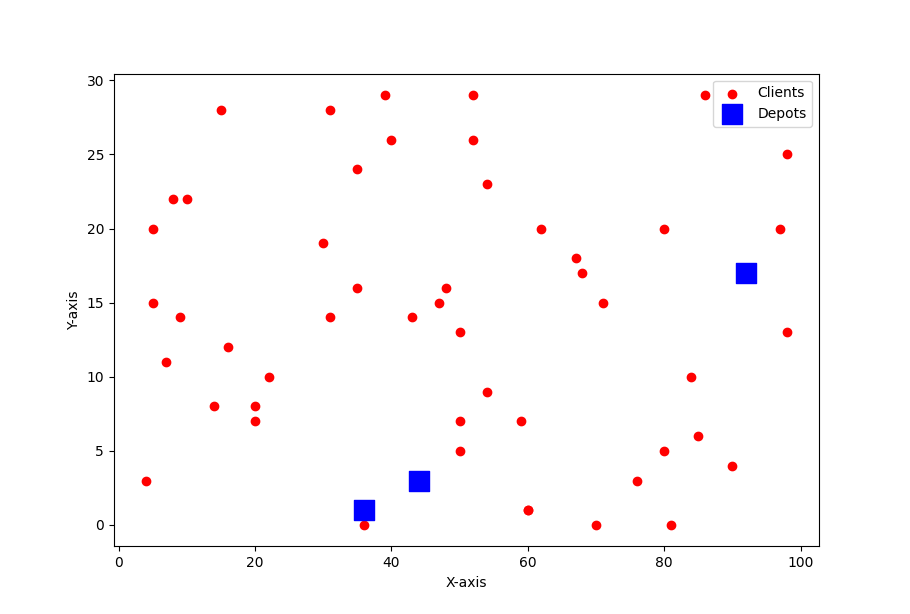
\includegraphics[width=\linewidth]{img/inst_1.png}
    \caption{Instância do problema}
    \label{fig:inst1}
  \end{figure}
  
  \subsection*{Estrutura de dados}
  \label{subsec:estruturadosdados}
  \textcolor{red}{A principal estrutura de dados utilizada nas heurísticas e nos modelos é dedicada à representação das plantas, onde podemos acessar em cada instante as viagens que são realizadas. Mais profundamente, corresponde a um vetor de tamanho igual ao horizonte de tempo, onde cada posição desse vetor armazenará as viagens que ocorrerão em cada um dos seus instantes. Por exemplo, caso a viagem 3 seja executada no período de 10 a 20, adicionaremos o valor 3 nas posições [10,20) do vetor. A quantidade de viagens em cada instante representa a quantidade mínima de veículos utilizadas por essa planta nesse instante. A maior quantidade de viagens simultâneas representará a quantidade de veículos utilizados pela planta. 
  Na imagem abaixo, vemos uma representação dessa estrutura de dados utilizada.}
  
  % \captionsetup{aboveskip=0pt,belowskip=1pt}
  \begin{figure}[H] % "H" ensures the figure stays in the exact place
    \centering
    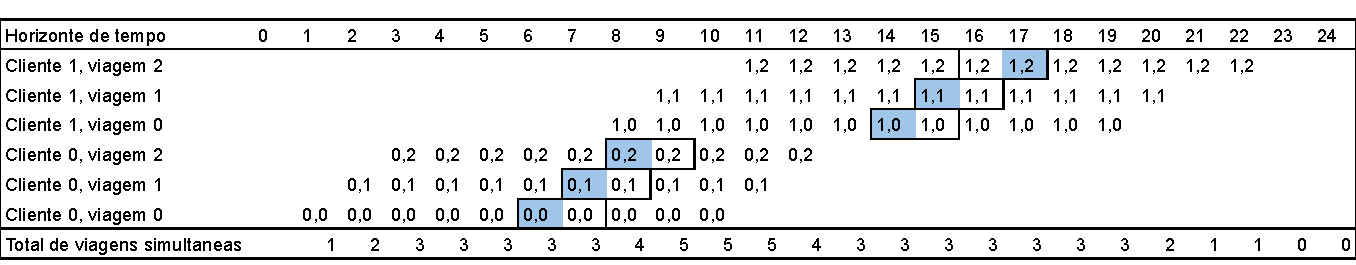
\includegraphics[width=1\textwidth]{img/estrutura de dados.pdf}
    \caption{Estrutura de Dados}
  \end{figure}
  
   \textcolor{red}{No exemplo da figura acima, temos a atribuição das viagens de dois clientes a uma planta. A janela de tempo para entrega é de duas unidades de tempo e estão com bordas nos instantes cuja entregas são permitidas. As viagens do cliente 0 custam 4 unidades de tempo para a ida e 4 unidades de tempo para a volta, enquanto as viagens do cliente 1 custam 6 unidades de tempo em cada sentido. Os instantes em azul indicam o momento das entregas.
  Nesse exemplo, a viagem 2 do cliente 1 foi executada no último instante da janela de tempo, fazendo assim com que a quantidade de viagens simultâneas no instante 10 não chegasse a seis, fazendo com que a necessidade de veículos nessa planta não superasse 5 em nenhum instante. }
   
	\renewcommand\bibname{Referências} %% Trabalhos em português
	% \renewcommand\bibname{References} %% Trabalhos em inglês
	\bibliographystyle{plain}
	\bibliography{99_referencias}
	% \chapter{Introdução}
	% Exemplo de nota de rodapé \footnote{Aqui está uma nota de rodapé e uma url: \url{https://dcc.ufmg.br}}.
		
		% \section{Motivação}
		% 	\lipsum[4-5]
			   
		% 	\subsection{Sub-motivação}
		% 		\lipsum[6-7]
		% 	\subsection{Mais uma sub-motivação}
		% 		\lipsum[8-9]
		% 		\subsubsection{Uma sub-sub-motivação}
		% 			\lipsum[10-11]
	
	% \chapter{Desenvolvimento}
	% 	\lipsum[1-4]
		
%		Exemplo de algoritmo ==============================
%		\begin{algoritmo}
%			\centering
%			\framebox[.5\textwidth]{\texttt{Código, Código, Código}}
%			\caption{Este é o meu Algoritmo 1.}
%			\label{alg:algoritmo1}
%		\end{algoritmo}
%	
%		\begin{algoritmo}
%			\centering
%			\framebox[.7\textwidth]{\texttt{Mais Código, Mais Código, Mais Código}}
%			\caption{Este é o meu Algoritmo 2.}
%			\label{alg:algoritmo2}
%		\end{algoritmo}
%		===============================================
		
		% \begin{figure}[ht]
		% 	\centering
		% 	\caption{Prédio do DCC em 2016.}
		% 	\label{fig:exemplo}
		% 	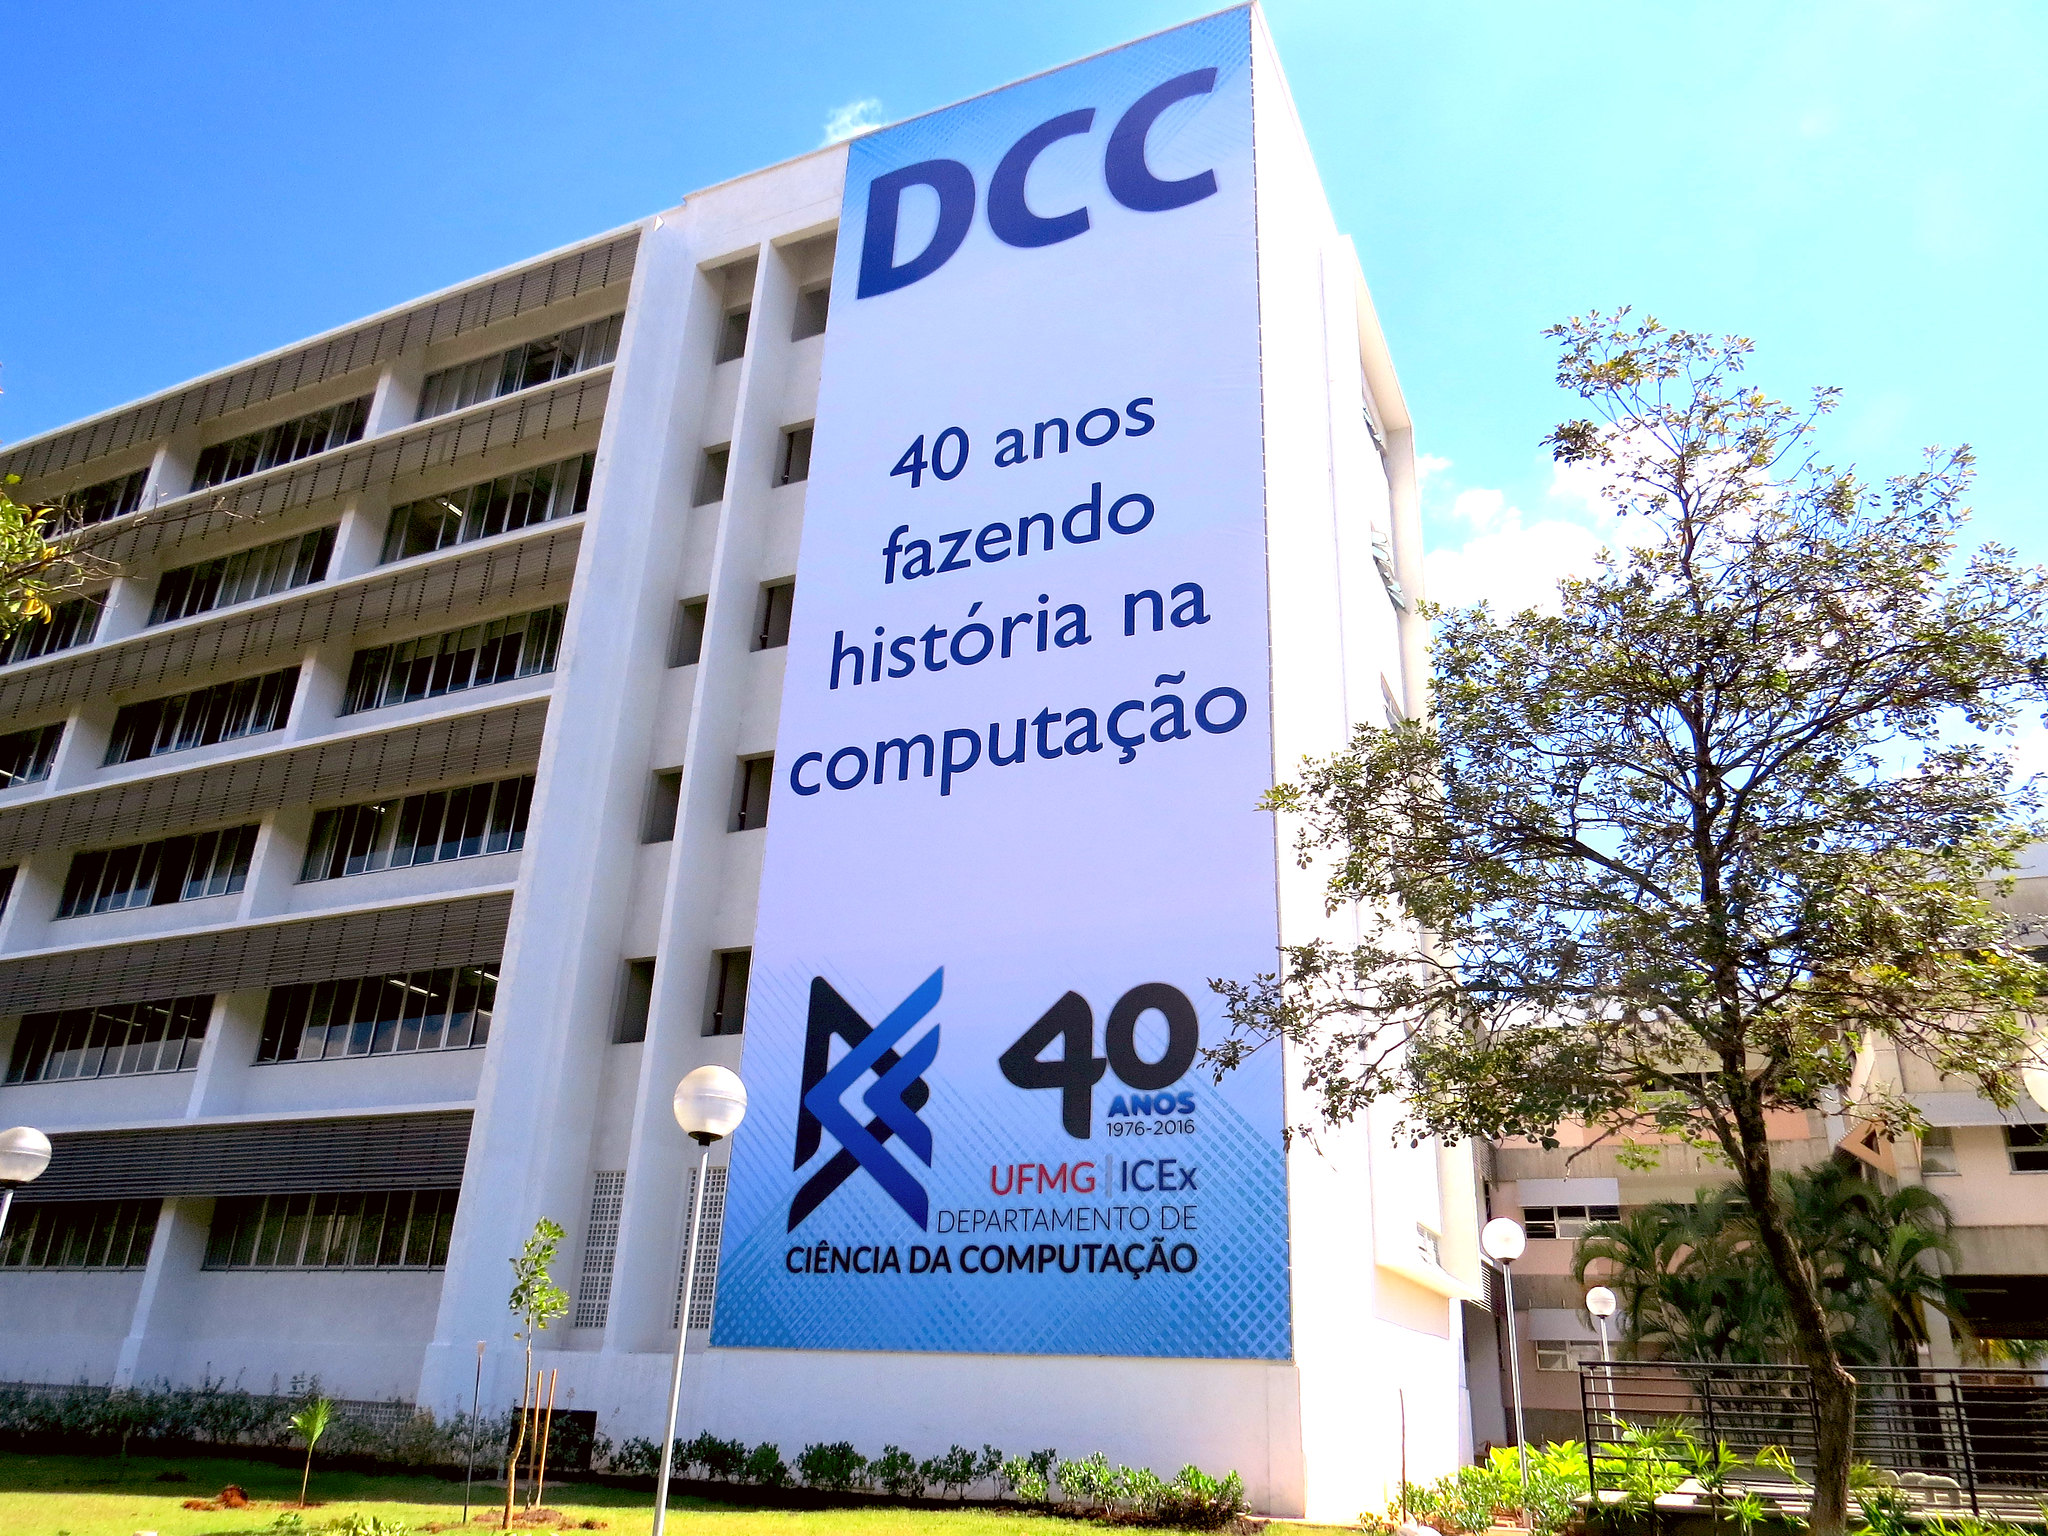
\includegraphics[width=\textwidth]{img/dcc.jpg}
		% 	\small{Fonte:~\url{http://40anos.dcc.ufmg.br/galeria}}
		% \end{figure}
	
		% \lipsum[5]
		
		% \begin{table}[ht]
		% 	\centering
		% 	\begin{tabular}{c|ccccccccl}
		% 		Natural & \multicolumn{9}{c}{Real}   \\ \hline
		% 		1 & 0.  & {\color{red} 2}  & 3   & 6   & 4   & 3   & 6   & 7   & $\ldots$ \\
		% 		2  & 0.  & 0   & {\color{red} 9}  & 8   & 4   & 7   & 3   & 2   & $\ldots$ \\
		% 		3  & 0.  & 1   & 9   & {\color{red} 3}  & 2   & 1   & 4   & 0   & $\ldots$ \\
		% 		4  & 0.  & 8   & 4   & 3   & {\color{red} 2}  & 7   & 9   & 2   & $\ldots$ \\
		% 		5  & 0.  & 0   & 1   & 2   & 9   & {\color{red} 3}  & 4   & 8   & $\ldots$ \\
		% 		6  & 0.  & 2   & 8   & 2   & 6   & 5   & {\color{red} 8}  & 3   & $\ldots$ \\
		% 		7  & 0.  & 0   & 2   & 1   & 5   & 3   & 7   & {\color{red} 4}  & $\ldots$ \\
		% 		$\vdots$ & $\vdots$  & $\vdots$  & $\vdots$  & $\vdots$  & $\vdots$  & $\vdots$  & $\vdots$  & $\vdots$  & $\ddots$ \\ \hline
		% 		\multicolumn{1}{l|}{} & \multicolumn{1}{l}{0.} & \multicolumn{1}{l}{{\color{red} 2}} & \multicolumn{1}{l}{{\color{red} 9}} & \multicolumn{1}{l}{{\color{red} 3}} & \multicolumn{1}{l}{{\color{red} 2}} & \multicolumn{1}{l}{{\color{red} 3}} & \multicolumn{1}{l}{{\color{red} 8}} & \multicolumn{1}{l}{{\color{red} 4}} & $\ldots$
		% 	\end{tabular}
		% 	\caption{Cantor: Existem infinitos diferentes!}
		% 	\label{tab:exemplo}
		% \end{table}

		% \section{Usando referências}
		% 	Segundo \cite{horn86robot}, todo triângulo equilátero tem os lados iguais. Já segundo \cite{shashua97photometric}, todo quadrado também tem.
			
		% 	Veja que o pacote \verb|natbib| permite uma série de formas diferentes para fazer referências bibliográficas. O comando padrão, \verb|\cite|, realiza a citação comum vista no parágrafo anterior. Outros comandos permitem, por exemplo, colocar automaticamente a citação entre	parênteses \citep{hougen93estimation, sato99illumination2, sato99illumination1, sato01stability}.
			
		% 	O comando usado foi \verb|\citep|. Veja a documentação do \verb|natbib| na Internet para conhecer	outros comandos e exemplos de uso.
			
		% 	Citações aleatórias para fazer com que as referências bibliográficas ocupem	mais de uma página: \cite{bichsel92simple, dror01statistics, guisser92new, dwork2006calibrating, sweeney2002k}.
			
		%% Referências
		
		% \begin{apendices}
		% 	\chapter{Um apêndice}
		% 		\lipsum[1-3]
				
		% 	\chapter{Outro Apêndice}
		% 		\lipsum[4-6]
				
		% \end{apendices}
		
\end{document}
